\documentclass{article}
\usepackage{listings}
\usepackage[utf8]{inputenc}
\usepackage{graphicx}
\renewcommand{\figurename}{Figura}
\usepackage{mathtools}
\usepackage{hyperref}
\usepackage[spanish]{babel}

\title{Informe de Estadística en Física Experimental: Ejercicio 9 Guía 3}
\author{Andr\'es Babino}

\begin{document}
\maketitle
\section{Introducción}
El lenguaje utilizado para programar todas los ítems fue Python.
El código utilizado para generar los datos, gráficos y este mismo informe fue controlado con git, tiene licencia MIT y está almacenado en \url{https://github.com/ababino/efe}.

\section{Ítem b}
$$f (x) = U(0, 1)$$
$$ g(y) = \lambda e^(-\lambda y)$$
$$g(y) \frac{dy}{dx} dx= f(x) dx $$

$$\lambda e^(-\lambda y) \frac{dy}{dx} = 1 $$

$$ y = -\frac{1}{\lambda} ln(1-x)$$

%\begin{lstlisting}
%def binomial_sample(n, p):
%    """
%    Takes a sample of size n from a binomial distribution with a success
%    probability equal p. Returns the number of sucesses.
%    """
%    s = 0
%    for i in xrange(n):
%        x = random.random()
%        if x < p:
%            s += 1
%    return s
%\end{lstlisting}

%\begin{figure}
%\centering
%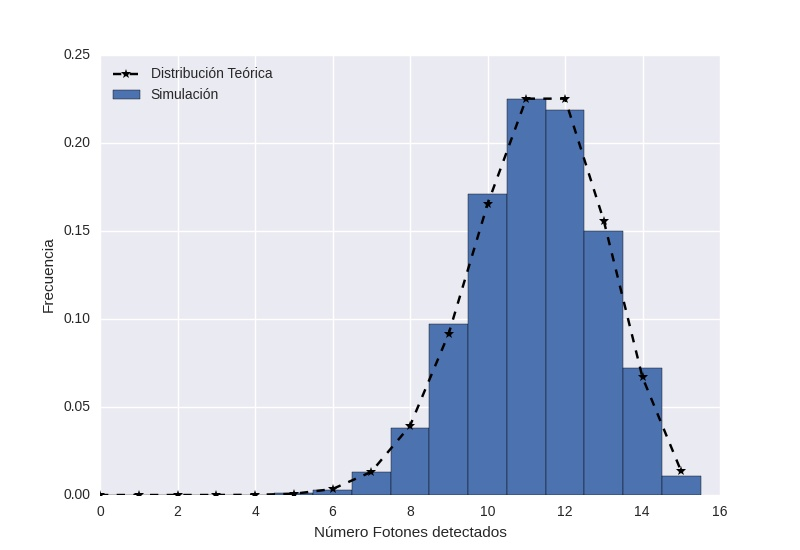
\includegraphics[width=0.75\textwidth]{figb.jpg}
%\caption[]{Histograma del ítem b}
%\label{fig:itemb}
%\end{figure}


\end{document}
